\chapter{Theory}
This thesis is placed in the field of \acrfull{hci}. Themes and methods used in this thesis, are therefore mostly connected to HCI.

The thesis is written with a Norwegian perspective in mind, and most theory, examples and data will therefore be in the context of Norway and the Norwegian population. 

\section{Interaction Design and \acrfull{hci}} 
\acrshort{hci} is an academic field concerned with "understanding the influence technology has on how people \textit{think, value, feel and relate}" and how this understanding can inform the design of technology \parencite{wright_empathy_2008}. Interaction Design is the industrial adaptation of HCI research, and is concerned with the practical design of products with the ultimate goal of supporting people (end users) in their everyday and working lives \parencite{rogers_interaction_2011}.

Both HCI and Interaction Design is concerned with understanding people and how they use ICT solutions and how the user experience can be improved in existing solutions or intact/integrated in future solutions.

%user experience

%empathy
%sympathy


\section{Regulations and guidelines}
In Norway, a regulation concerning Universal Design was passed in 2013 (Kommunal- og moderniseringsdepartementet, 2013). According to \Gls{difi} the vision of having this regulation is to have a society without digital barriers \parencite{difi_digitale_2015}. Digital barriers refers to the hinderings some people with impairments experience using technology, and it comes according to \textcite{malin_rygg_dei_2015} mostly from bad coding, low contrast and lack of textual alternatives for illustrations on websites. 

\subsection{Discrimination and Availability Act}
The Norwegian legislation "Discrimination and Availability Act" (no: Diskriminerings- og tilgjengelighetsloven) came in effect 1. January 2009. The legislation states that "equality, equal opportunities and community engagement should be available to all, independent on functional abilities". The law also makes sure to hinder discrimination because of disabilities.

According to the legislation, ICT-solutions that are aimed at the public must be universal designed by 1. Juli 2011. Existing solutions must be universal designed by 1. January 2021 \parencite{_lov_2013}. Failure to meet this deadline might result in a coercive fine \parencite{_lov_2013}.

\subsection{WCAG 2.0 guidelines}
The extent to if, and how well universal designed a website or application is, is in Norway measured by using the \Gls{WCAG} (Web Content Accessibility Guidelines) 2.0 technical standard. Norwegian websites (and some applications) that are aimed at Norwegian citizens, are used to inform or offer services, and is new or published after 1. July 2014, are all affected by this regulation. Providers of websites and applications that are older than this have until 1. January 2021 to meet the WCAG 2.0 requirements (ibid).
\Gls{WCAG} is based on four top principles:
\begin{itemize}
    \item Perceivability
    \item Operability
    \item Understandability
    \item Robustness
\end{itemize}

Under these principles are guidelines that explain the goals each success criteria should meet. WCAG 2.0 includes testable success criterion in three levels: A, AA and AAA, which are separated in the degree the success criterion impacts the design of the website. Most AA success criterion are included in the regulation on universal design of ICT solutions. %cite the regulation


\section{Definitions and wording}
\subsection{Sympathy vs. empathy}
Empathy can be described as "understanding the other and seeing a situation from the perspective of others" \parencite{lundstrom_perceptions_2015}.  

%skriv om hvordan man får til empati etc.

%\textcite{wright_empathy_2008} notes that the first view of empathy, identify and becoming the user, 


\subsection{Accessibility and Universal Design}
Accessibility and Universal Design are related terms. Accessibility is concerned with whether a solution has the properties of being usable by people with impairments. \textcite{paddison_applying_2003} separates technical and usable accessibility. Technical accessibility is making sure the solution are usable by assistive technology, such as screen readers, by adding alternative text, using scalable measures in font sizes et cetera. Usable accessibility is ensuring a good user flow, consistent layout and more.

When ICT-solutions are accessible \textit{and} usable (that it governs both technical and usable accessibility) to a larger part of the population, it is often referred to as being “Universally Designed”. The Norwegian Environmental Protection Agency defined Universal Design in 2007 as “...the design of products and environments to be usable by all people, to the greatest extent possible, without the need for adaptation or specialised design” \parencite{miljoverndepartementet_t-1468_2007}. This means that the same solution should be usable for people with different functional levels. 

As an example: if a website with 500 links is accessible with the use of a screen reader, it can be said to be accessible. If the same website is usable for the people using the screen reader, without them having to go through all the 500 links to execute a task, it can be said to be Universal Designed. 

This is an oversimplification of the terms, and it all depends on the user, their abilities, the technology, the setting the technology is used and many other factors. Universal Design of ICT has the ultimate goal of making ICT accessible and usable for a given target group in an appropriate way \parencite{tollefsen_web_2013}, and to lower the digital barriers of the society. 

%\textcite{tollefsen_web_2013} defines Universal Design of ICT as “...development of products and services so that all people in a given target group can use the technology in an appropriate way”.

%In Norway, a regulation concerning Universal Design was passed in 2013 (Kommunal- og moderniseringsdepartementet, 2013). According to \Gls{difi} the vision of having this regulation is to have a society without digital barriers \parencite{difi_digitale_2015}.

%\Gls{UniversalDesign} as a concept began, according to \textcite{tollefsen_web_2013} at The Center for Universal Design at the end of 1980s. In Norway it began with the publication "Universal Design - planning and design for all" from 1997. %\gls{disability}.


\subsection{Disability and impairments}
Most people, especially in Norway, can expect access to education, employment, public transport and information. This is not necessarily the case for people who live with disabilities. According to \textcite{world_health_organization_world_2011} around 15\% of the world's population live with some sort of disability. This number is also growing because people are generally getting older, and older people have a higher risk of being disabled. 

\acrfull{ffo} defines disability as a conflict between an individuals premise to function and the environments requirements to function \parencite{funksjonshemmedes_fellesorganisasjon_ffo_definisjon_2013}. The Gap Model \ref{fig:gap_model} illustrates this conflict: 
\begin{figure}[H]
\minipage{1\textwidth}
  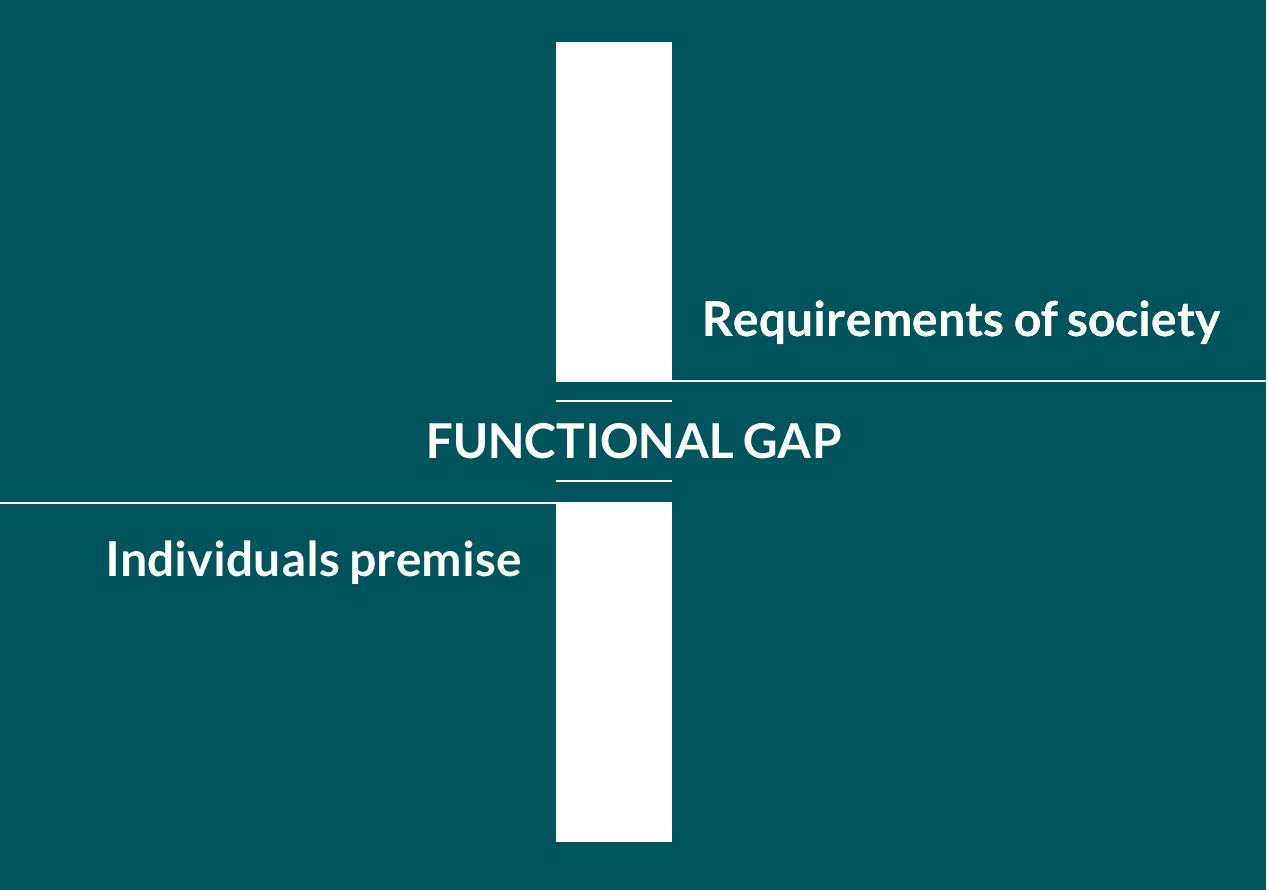
\includegraphics[width=\linewidth]{img/gapmodel.png}
  \caption{The Gap Model. Graphic based on \textcite{difi_kvifor_2016}.}\label{fig:gap_model}
\endminipage\hfill
\end{figure}
In order to decrease the functional gap, requirements of the society must be lowered. A way of doing this is to make sure ICT solutions are universally designed so that most people are able to participate in society. 
It is important to distinguish the terms "disability" and "impairment" as these are often used interchangeably \parencite{sheena_l._carter_impairment_????}. \textbf{Impairment} refers to "any loss or abnormality of psychological, physiological or anatomical structure or function." while \textbf{disability} refers to "any restriction or lack (resulting from an impairment) of ability to perform an activity in the manner or within the range considered normal for a human being" (ibid). 

More clearly, \textbf{impairment} refers to the \textit{physical} or \textit{cognitive} hindering/restriction of functionality the individual may have, while \textbf{disability} refers to the restriction the individual have to perform certain \textit{activities} or \textit{tasks}, because of the impairment. With this definition in mind, one can say that inaccessible environments \textbf{disables people} with impairments, not that the person are disabled because of their impairment. \textcite{world_health_organization_world_2011} also discusses this idea using the models "medical" and "social" where medical are the impairments the person may have, while the social model refers to the hinderings caused by society (the functional gap).

\subsection{Universal Design, Inclusive Design and all the above}

\iffalse
    \section{Disabilities and impairments}
    Most people, especially in Norway, can expect access to education, employment, public transport and information. This is not necessarily the case for people who live with disabilities. According to \textcite{world_health_organization_world_2011} around 15\% of the world's population live with some sort of disability. This number is also growing because people are generally getting older, and older people have a higher risk of being disabled. 
    
    \acrfull{ffo} defines disability as a conflict between an individuals premise to function and the environments requirements to function \parencite{funksjonshemmedes_fellesorganisasjon_ffo_definisjon_2013}. The Gap Model \ref{fig:gap_model} illustrates this conflict: 
    \begin{figure}[H]
    \minipage{1\textwidth}
      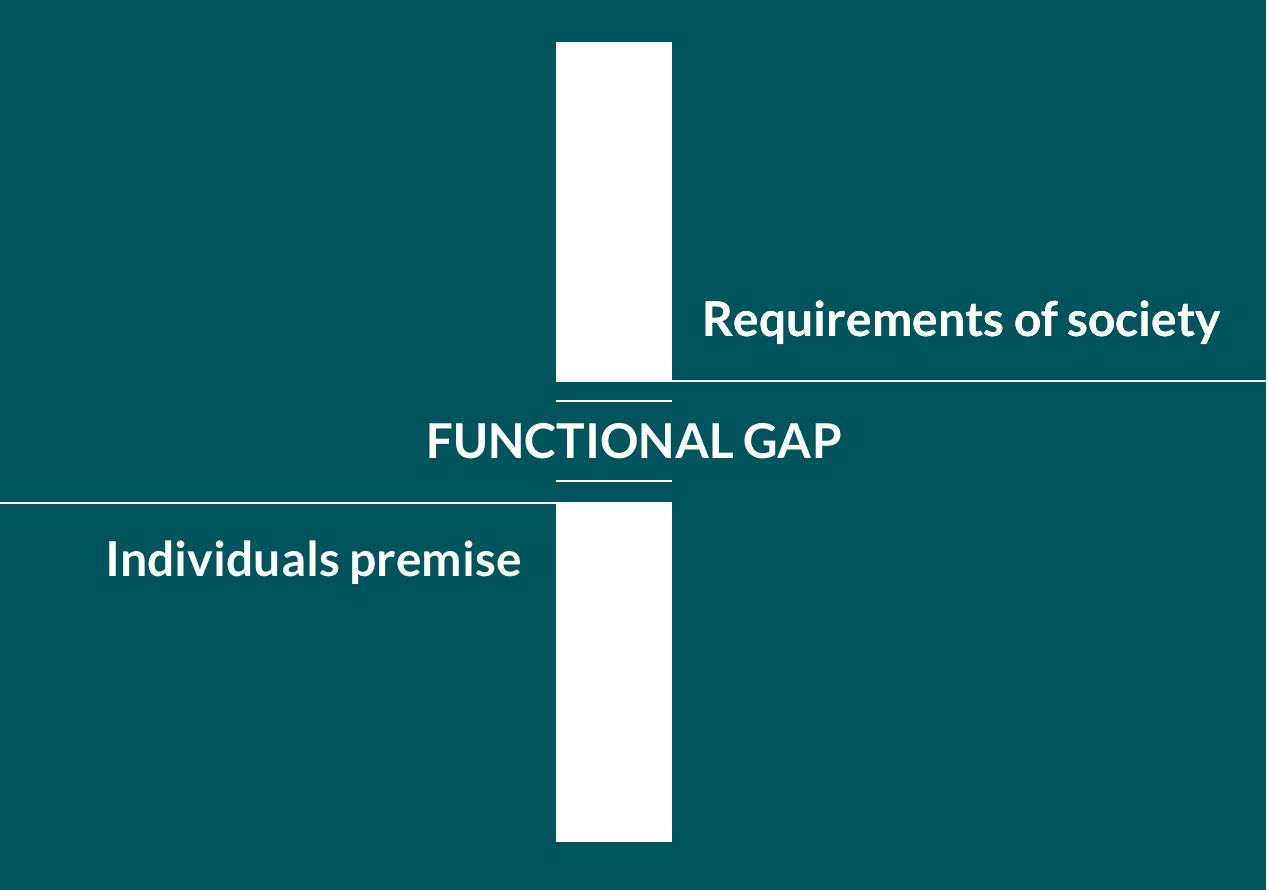
\includegraphics[width=\linewidth]{img/gapmodel.png}
      \caption{The Gap Model. Graphic based on \textcite{difi_kvifor_2016}.}\label{fig:gap_model}
    \endminipage\hfill
    \end{figure}
    
    In order to decrease the functional gap, requirements of the society must be lowered. A way of doing this is to make sure ICT solutions are universally designed so that most people are able to participate in society. 

\fi

\subsection{Impairments and disabilities}
It is important to distinguish the terms "disability" and "impairment" as these are often used interchangeably \parencite{sheena_l._carter_impairment_????}. \textbf{Impairment} refers to "any loss or abnormality of psychological, physiological or anatomical structure or function." while \textbf{disability} refers to "any restriction or lack (resulting from an impairment) of ability to perform an activity in the manner or within the range considered normal for a human being" (ibid). 

More clearly, \textbf{impairment} refers to the \textit{physical} or \textit{cognitive} hindering/restriction of functionality the individual may have, while \textbf{disability} refers to the restriction the individual have to perform certain \textit{activities} or \textit{tasks}, because of the impairment. With this definition in mind, one can say that inaccessible environments \textbf{disables people} with impairments, not that the person are disabled because of their impairment. \textcite{world_health_organization_world_2011} also discusses this idea using the models "medical" and "social" where medical are the impairments the person may have, while the social model refers to the hinderings caused by society (the functional gap).


\textcite{begnum_universal_2017} also mentions this difference between the medical and social model, where the medical model are concerned with what is wrong with a person, while the social model is concerned with what is wrong with society the individual is a part of. She says "it is a \textbf{social responsibility} to ensure that different physical and psychological abilities are taken into consideration and barriers are removed and diminished". 



%få med modell fra Jo - Gdrive

\subsection{Types of disabilities}
\Gls{difi} categorises four main groups of disabilities and how they can hinder people from using technology:
\begin{itemize}
    \item Motoric 
    
    Disabilities regarding movement and motorics. People in this category are sometimes in need of other types of interaction methods other than mouse, touch screen, keyboard or buttons in order to operate digital devices; for example eye tracking, joysticks or other alternative interaction methods.
    \item Visual
    
    People who experience visual impairments are people who, to some degree, have problems seeing or who are totally blind. This group consists of people with, amongst others, colour blindness, blurred vision or poor eyesight. 
    
    People with visual impairments can have problems with small text, small touch/click areas, unusual fonts etc. This group can also struggle when colours are the only differentiating factor between elements, or when contrast between elements are too low. 
    \item Auditory
    
    Auditory impairment refers to having problems hearing or being deaf. People with auditory impairments can have problems hearing the audio track of videos, sound clips or music, and needs the information presented textual or with sign language. 
    
    \item Cognitive
    
    This category involves people with problems processing information. Cognitive impairments involves: memory problems, concentration problems, learning problems, literacy problems etc. This group can be in need of other information
\end{itemize}

However, as noted by \textcite[p. 22]{world_health_organization_world_2011} people with the same type of impairment may have different experiences and needs. \\ 

%\textbf{SKRIV MER OM DETTE}

\noindent
In the Norwegian population:
\begin{itemize}
    \item 15\% in 2017 says they have impairments \parencite{barne-_ungdoms-_og_familiedirektoratet_antall_2017}
    \item [\textbf{Vision}]
        \item 180.000 live with a vision impairment \parencite{blindeforbundet_fakta_????}
        \item Over 1000 are color blind \parencite{blindeforbundet_fakta_????}
        \item 70\% of people over 70 develops cataracts \parencite{blindeforbundet_fakta_????}
    \item [\textbf{Cognitive}]
        \item 2.5\% adults has ADHD \parencite{adhd_norge_voksen_????}
        \item Around 5\% has dyslexia, 5\% has dyscalculi and 5\% has SSV \parencite{dysleksi_norge_fagstoff_????}
    \item [\textbf{Language}]
        \item 725.000 are first generation immigrants which most likely has another mother tongue than Norwegian \parencite{statistisk_sentralbyra_nokkeltall_2017}
    \item [\textbf{Age}]
        \item 220.000 people in 2017 are 80 years or older, 505.000 people are between 75 and 79 years old \parencite{folkehelseinstituttet_andelen_2017}
\end{itemize}
These statistics show that there is a large amount of the Norwegian population who lives with different kinds of impairments. \\

\noindent
Everyone will most likely experience some sort of physical or cognitive impairment \parencite{world_health_organization_world_2011} hindering them from using technology and accessing information. Everyone will get older, and considering the increased focus on digitisation of the public services, Universal Design will be an important tool to ensure that most people will be able to participate in society. 

%The information provided must be available to everyone regardless of software, platform, environment or ability \parencite{paddison_applying_2003}.

% \section{Empathy}

% \parencite{wright_empathy_2008} discusses qualitative methods for \textit{eliciting or evoking experiences}.

% \section{University of Cambridge's impairment simulator software}
% To provide a way to empathise with people having different disabilities, Cambridge University has developed a set of simulation tools they call "Capability loss simulation". The simulation toolset consists of glasses and software that simulates vision impairments and gloves which simulates fine motor-impairments (such as arthritis).

% The article ”Equipping Designers by Simulating the Effects of Visual and Hearing Impairments” by Goodman-Deane et al. discusses the impairment simulator software made by University of Cambridge.

% %The authors claim that although inclusive design provides great benefits for every user of the end product, this can be difficult to achieve in practise. It can be hard to understand the diversity of needs users with different disabilities have, and to estimate the impact different design decisions have on these user groups. Using simulations, some of these obstacles may be overcome.

% \begin{figure}[H]
% \minipage{0.8\textwidth}
%   \includegraphics[width=\linewidth]{src/img/cambridge_simulator.jpg}
%   \caption{The interface of the Cambridge Capability Loss simulator. Diabetic Retinopathy is selected.}\label{fig:cambridge_simulator_interface}
% \endminipage\hfill
% \end{figure}


\section{Evaluating accessibility}
\textcite{bai_evaluation_2016} identifies four ways of testing accessibility:
\begin{itemize}
    \item Automatic and semi-automatic testing using tools and guidelines
    
    Tools used to compare against a checklist or guideline. Automatic tools \textcite{bai_evaluation_2016} lists are modules included in a developer enviroment such as NetBeans, which gives automatic feedback whether the code used is in line with accessibility guidelines. They also include software simulation tools such as the NoCoffee chrome extension to simulate vision impairments and tools to simulate dexterity (hand coordination) impairments.
    
    \begin{figure}[H]
        \minipage{1\textwidth}
          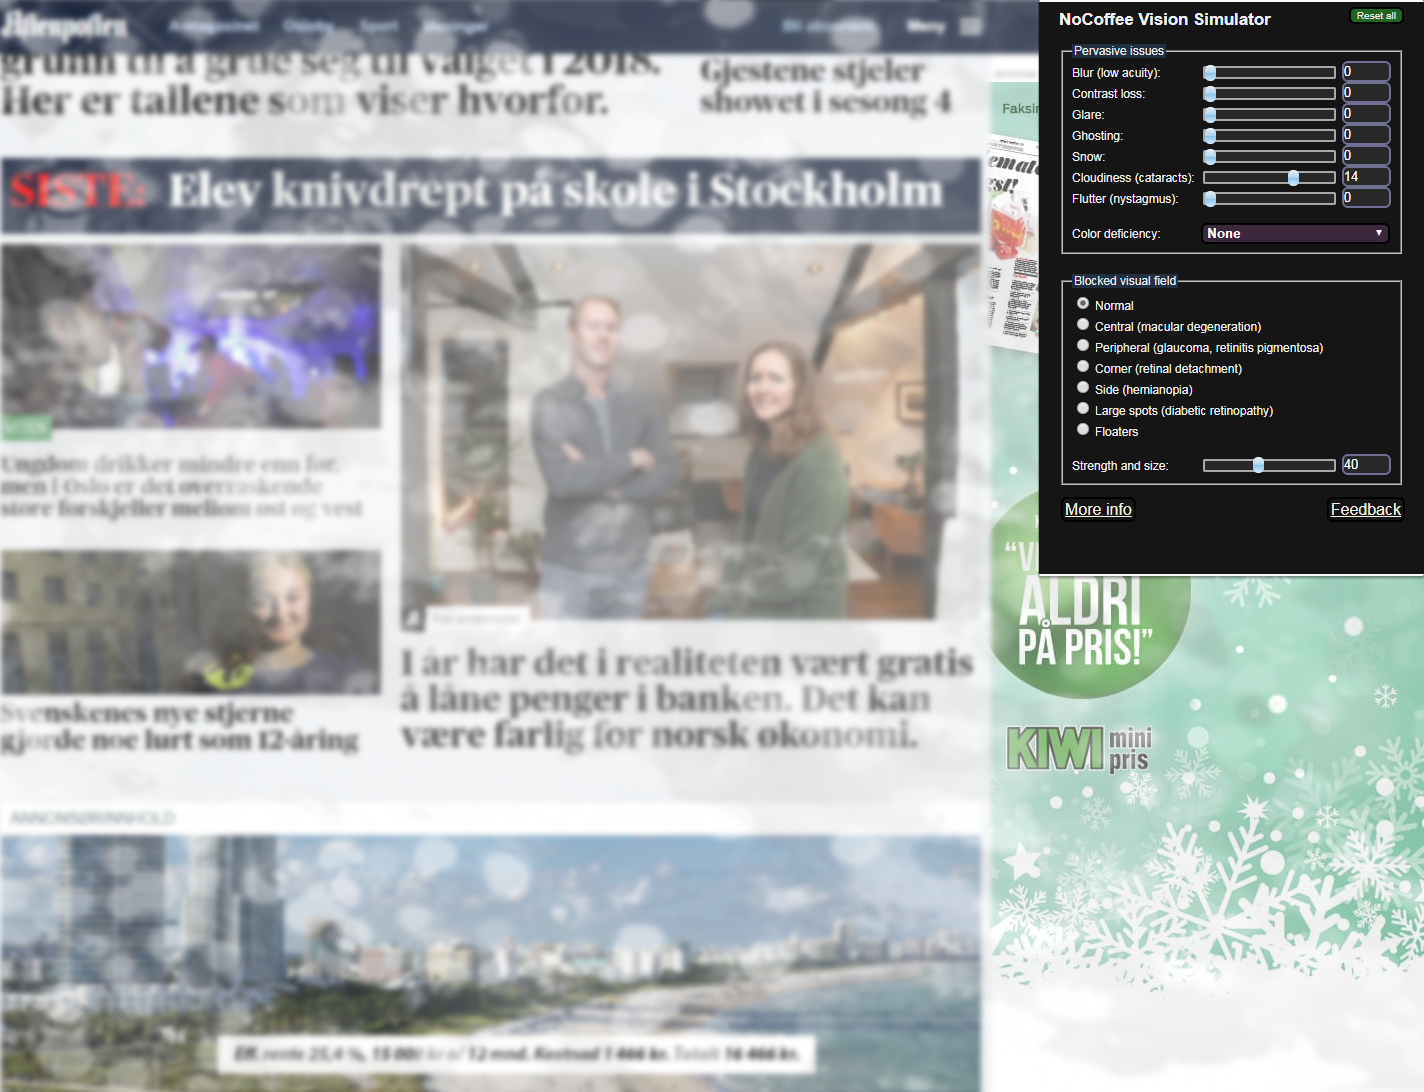
\includegraphics[width=\linewidth]{img/nocoffee.PNG}
          \caption{\textit{The Chrome extension "NoCoffee" simulates different vision impairments by adding a filter on the screen.}}\label{fig:nocoffee_browser_extension_theory_1}
        \endminipage\hfill
    \end{figure}
    \item Simulation using wearable
    
    Vision impairment simulators such as Cambridge simulation glasses and Blue Label Goggles, gloves for simulating dexterity impairments and earplugs for simulating hearing impairments.

    % take own images of cambridge glasses and insert here    
    % \begin{figure}[H]
    %     \minipage{0.8\textwidth}
    %       \includegraphics[width=\linewidth]{src/img/cambridge_simulator.jpg}
    %       \caption{The interface of the Cambridge Capability Loss simulator. Diabetic Retinopathy is selected.}\label{fig:cambridge_simulator_interface}
    %     \endminipage\hfill
    % \end{figure}
    \item Expert testing
    
    Heuristic evaluation where experts evaluates a UI against a set of accepted accessibility heuristics/principles. The authors also includes persona walk-through and cognitive walk-through.
    
    \item Testing with users
    
    Testing a UI on real people. The authors claims that it can be time consuming to recruit subjects and that the most critical accessibility flaws needs to be solved before involving users. 
\end{itemize}

In this thesis I will focus on experience based software simulation, a mixture of \textcite{bai_evaluation_2016}'s "automatic" and "simulation using wearable". More on this in section \ref{discevalsect}.

\section{Universal Design in ICT projects}
\textcite{fuglerud_link_2013} states that although guidelines such as WCAG 2.0 is a precondition to achieve an accessible solution, it might not always be enough. A solution might be technically or theoretically within the requirements of universal design, but still be difficult to use. Some research suggests that WCAG 2.0 only covers around half  of the issues encountered by visually impaired users \parencite{fuglerud_link_2013}.

In the past decade, there has been an increased focus on integrating usability in the software development process \parencite{bai2017cost}. Usability is the focus of the quality and the ease of use of a product. Many companies see the value in making sure their products are user friendly,  and spends resources on usability testing in ICT projects, even though usability testing can take around 8-13\% of the total budget of the project \parencite{bai2017cost}. The incentive for doing this can be that solutions which are difficult to use or are hard to understand makes the user find better alternatives. 

\textcite{bai2017cost} argues that the same focus should be on accessibility testing, even though the cost for user testing for accessibility can be higher then testing for usability, because of the recruitment and accommodation of people with various forms of disabilities can be harder.  

\textcite{fuglerud_link_2013} also argues that projects who has a goal of meeting universal design guidelines should follow a user-centered design methodology. They categorise key elements for having an inclusive design process:
\begin{itemize}
\item "Include multidisciplinary skills and perspectives, 
\item adapt and apply accessibility guidelines and standards,   
\item iterative development, 
\item focus  on  users  with  diverse  accessibility  needs  and  their  usage  contexts  early  and  
\item throughout the development process, 
\item evaluate designs with elderly and people with disabilities, and 
\item focus on the whole user experience."
\end{itemize}


In a utopian project, both usability testing and accessibility testing using real users are done, making sure the solution is user-friendly and accessible for as many people as possible. In reality, time and budget constraints can make it hard to integrate accessibility user testing in projects \parencite{bai_evaluation_2016}. 

\section{Simulations}
\textcite{GoodmanDeane:2007it} claims that although inclusive design provides great benefits for every user of the end product, this can be difficult to achieve in practise. It can be hard to understand the diversity of needs users with different disabilities have, and to estimate the impact different design decisions have on these user groups. Using simulations, some of these obstacles may be overcome.

\subsection{Software simulations}
Software simulation of impairments can demonstrate the effects some impairments have while using screen-based devices. According to \textcite{GoodmanDeane:2007it} software simulators can "help the designers to understand and empathise with the difficulties that less able users might experience when using their products and interfaces". 

\subsection{Critique on using simulators}
\textcite{GoodmanDeane:2007it} is clear on the fact that simulation does not convey the long-term limitations of living with a visual or hearing impairment, such as frustration or coping strategies, but it can give a short insight into the functional experience of having such an impairment. According to \textcite[3]{bai_evaluation_2016}, "the lack of awareness about this distinction is why this approach (simulations) has been highly criticized". 

\textcite{GoodmanDeane:2007it} also states that simulations should not be seen as a substitute for real user involvement, but as a way to internalise insight findings and to test a system before real users are involved. 

\subsubsection{Moore's age experiment}
Patricia Moore, which was in her twenties at the time, toured North America between 1979 and 1982 disguised as an old woman. She experienced abuse, discrimination and marginalisation. She was attacked on the street and on a flight an air hostess spilled coffee on her without apologising \parencite{coleman_design_2007}. 


%\subsection{Who should focus on Universal Design?}




% \section{How ICT solutions are developed}
% To figure out why ICT solutions are inaccessible, we have to understand how ICT solutions are 

% Dong et al. identifies two barriers to the adaption of inclusive design practises within industri in the UK. This study was on 


% Begnum states that there are two different approaches to work with universal design, and calles these "cultural stance": the first cultural stance is viewing  

% Begnum has studied how Universal Design is approached by Norwegian experts working on ICT solutions. She suggests that  there seems to be two cultural stances among the experts: technological and user-oriented. The technological stance, she writes, are more oriented towards checklists, automatic tests and expert inspections, while the 

\iffalse

    \section{Programmer-Focused Website Accessibility Evaluations}
    \begin{displayquote}
    "If you want to change some existing code, you have to first change the programmer's mind."
    \end{displayquote}
    
    %This article by \parencite{Law:ProgrammerFocusedWebsiteAccessibilityEvaluations:2005} highlights the need to treat programmers as the end-users of reports made by accessibility specialists, and it is up to them if the recommendations is implemented or not. These recommendations are often overlooked, if they are not "quick fixes". Programmers generally have a tight schedule and have little training in accessibility, so they only see these recommendations as extra work.
    
    %The authors have come up with a process which can overcome the obstacles, called Streamlined Evaluation and Reporting Process for Accessibility (SERPA). It begins by having the accessibility specialist discussing the project goals and needs of the involved members. The reason to do this is to tailor the future recommendations to the team members. The next step is to agree upon the scope of the project. The authors says it is better to focus on, for example, level A of the WCAG-standard. Next step is to generate a programmer-centric report including fixes first, then guidelines. This makes it easier to focus on the website, not the guidelines. Step four includes evaluating the website with screen readers and similar tools. The article is not clear on whether this means to include developers as evaluators.
    
    This article by \textcite{Law:ProgrammerFocusedWebsiteAccessibilityEvaluations:2005} highlights the problem of having accessibility experts suggesting accessibility fixes, normally in long reports, that are not meeting the needs of the programmers that actually implements the fixes. As a result, most suggestions are overlooked. 
        
    The article also suggests a process that considers the whole development process as well as interpersonal characteristics between programmers and managers. The process is programmer-centric and called "Serpa" (Streamlined Evaluation and Reporting Process for Accessibility).
    
    The ultimate goal of any project that is aimed at a wide population (including people with disabilities) is to be usable for the end-user. But the end user of accessibility reports and recommendations are programmers, and therefore these mediums needs to be usable for this target group. 
    
    Programmers usually have these characteristics:
    \begin{itemize}
        \item Little to no usability training
        \item Think web-users thinks like them
        \item Have little time, and have many groups fighting for their attention and time to fix bugs, aesthetic fixes, usability fixes etc.
        \begin{itemize}
            \item A report with thousand small fixes are less likely to be taken into consideration
        \end{itemize}
        \item Management, not accessibility experts, are more respected and taken serious because they are in charge of promotions and raises and should therefore be the ones in charge of which fixes should be implemented.
    \end{itemize}
    
    The article suggests that it is easier to change the programmers way of thinking then it is to get them to implement accessibility fixes. It is also highlighted that incorporating fixes from the beginning rather than retrofitting (fixing accessibility issues that already are in production), are much better, but that this article is concerned with retrofitting, as this is what most accessibility experts are involved with today.
    
    The last part of the article suggest a programmer-focused process called SERPA. The main parts of this process is:
    \begin{itemize}
        \item Discuss the needs and project goals with all team members.
        \item Agree on the scope and resources.
        \item Fixes could be based on some of the parts of the WCAG Guidelines but not all.
        \item Prepare a programmer-centric report template.
        \item Suggested fixes should be clear first, not accessibility guidelines.
        \item Separate fixes based on content and fixes based on the code / implementation.
        \item Alternative tags are a responsibility of content-creators, not programmers.
        \item Presenting content-related fixes to programmers may be counter-productive.  
    \end{itemize}
    
    \subsection{Outtakes} 
    This article can give me some insight into how some developers think, and how to make accessibility issues relevant to them. It can help me to make design decisions, and to formulate suitable questions for interviews.

\fi
\section{Existing solutions}
\subsection{Cambridge University Capability loss simulation toolkit}
To provide a way to empathise with people having different disabilities, Cambridge University has developed a set of simulation tools they call "Capability loss simulation". The simulation toolset consists of glasses and software that simulates vision impairments and gloves which simulates fine motor-impairments (such as arthritis).

\subsubsection{Impairment simulation software} \label{Impairment simulation software}
The impairment simulation software is making it easy to simulate hearing and vision loss. It includes a set of example pictures and audio files. The software simulates four levels of hearing loss, and several visual impairments and conditions. It is also possible to import pictures into the software, but they have to be of a specific file type. 

\begin{figure}[H]
\minipage{1\textwidth}
  \includegraphics[width=\linewidth]{img/cambridge_simulator.jpg}
  \caption{\textit{The interface of the Cambridge Capability Loss simulator. Diabetic Retinopathy is selected.}}\label{fig:cambridge_simulator_interface}
\endminipage\hfill
\end{figure}

\subsubsection{Cambridge simulation glasses}
In the same toolkit as the \nameref{Impairment simulation software} is the "Cambridge simulation glasses" which are meant to simulate vision loss. The glasses blurries the vision of the user, and can provide a way of experiencing how a person with vision loss might experience an interface. The glasses comes in packages of five or 30 pieces, and are meant to be used on top of each other to provide three different levels of vision loss impairment.

\subsection{NoCoffee browser extension}
NoCoffee is a simulator which can be used to simulate different vision impairments. It works by adding a filter on top of the content of the browser interface. The user of the simulator can adjust different settings such as degrees of blurring, ghosting, different types of color blindness etc.
\begin{figure}[H]
\minipage{1\textwidth}
  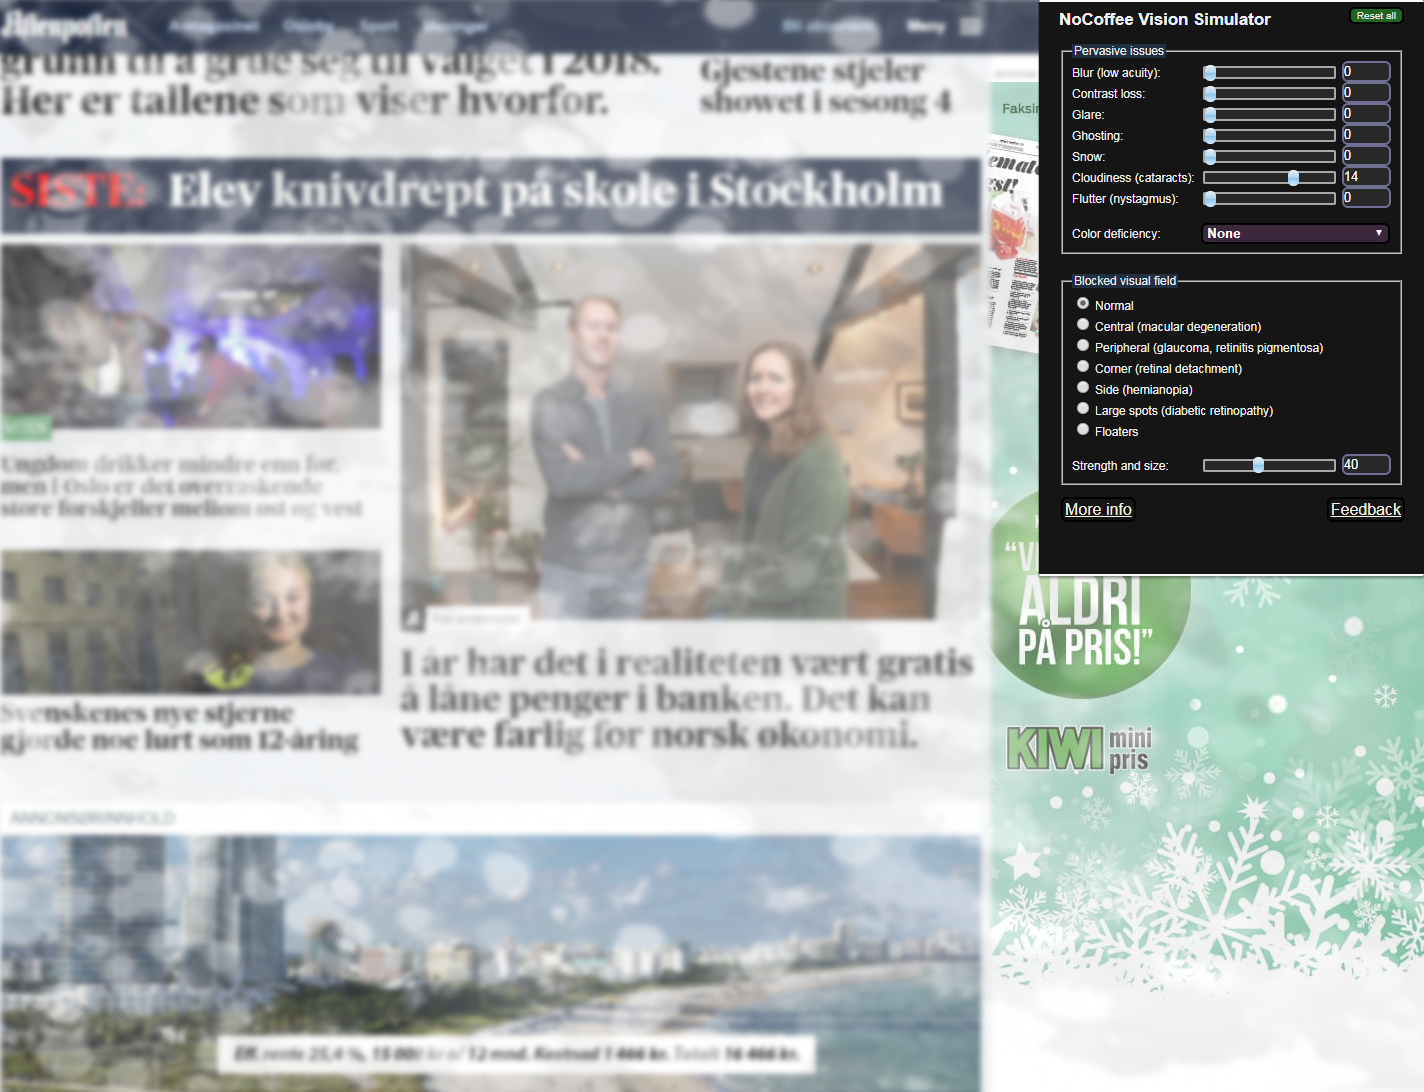
\includegraphics[width=\linewidth]{img/nocoffee.PNG}
  \caption{\textit{The Chrome extension "NoCoffee" simulates different vision impairments by adding a filter on the screen.}}\label{fig:nocoffee_browser_extension_theory_2}
\endminipage\hfill
\end{figure}

The maker of the simulator has posted some thoughts on limitations of the simulator \parencite{_nocoffee_2013}:
\begin{itemize}
    \item The simulations are not medically/scientifically accurate.
    \item The simulations of partial visual fields cannot follow your eyes.
    \item Settings are not linked to statistics and can be hard to relate to
    \item The simulator only works in Chrome
\end{itemize}

\subsection{Funkify browser extension}
This simulator is personas based, meaning that each setting is based on an imaginative person who has a certain impairment: "Blurry Blanca" has blurry vision, "Dyslexia Dani" has dyslexia and "Color Carl" is color blind. The simulator has eight different profiles, all portraying different kinds of impairments.
\begin{figure}[H]
\minipage{1\textwidth}
  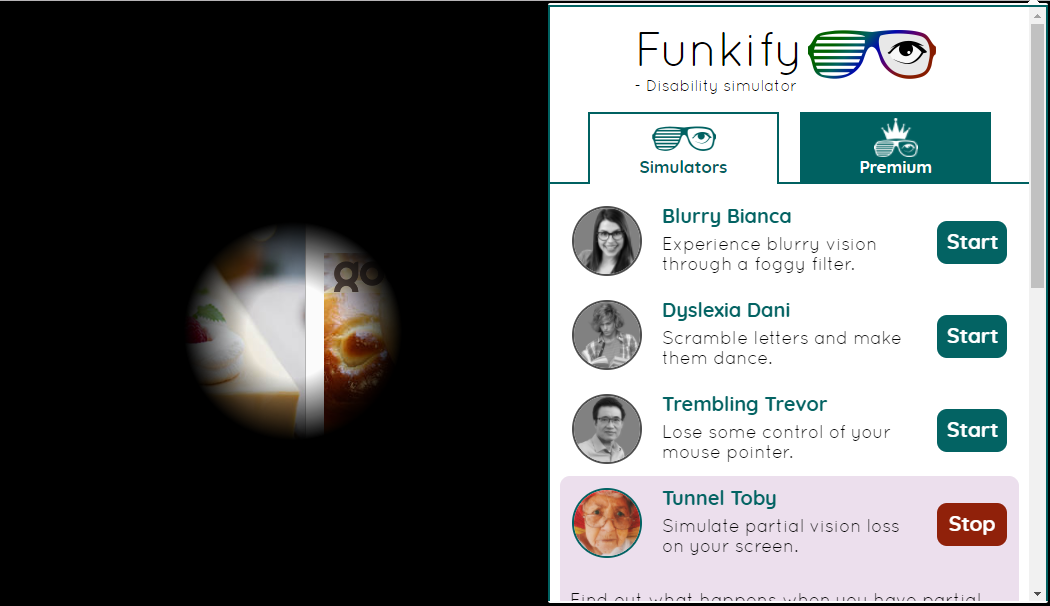
\includegraphics[width=\linewidth]{img/funkify.png}
  \caption{\textit{The Chrome extension "Funkify" simulates different vision impairments and showcases them using personas. Selected are "Tunnel Toby" simulating tunnel vision. The tunnel vision follows the mouse.}}\label{fig:funkify_tunnel}
\endminipage\hfill
\end{figure}
The simulator is created by usability and accessibility experts in Sweden and financed by The Swedish Post and Telecom Authority \parencite{funkify.org_funkify_????}\\

\noindent
The simulator provides statistics on how many people are effected on most of the disability personas.
\begin{figure}[H]
\minipage{1\textwidth}
  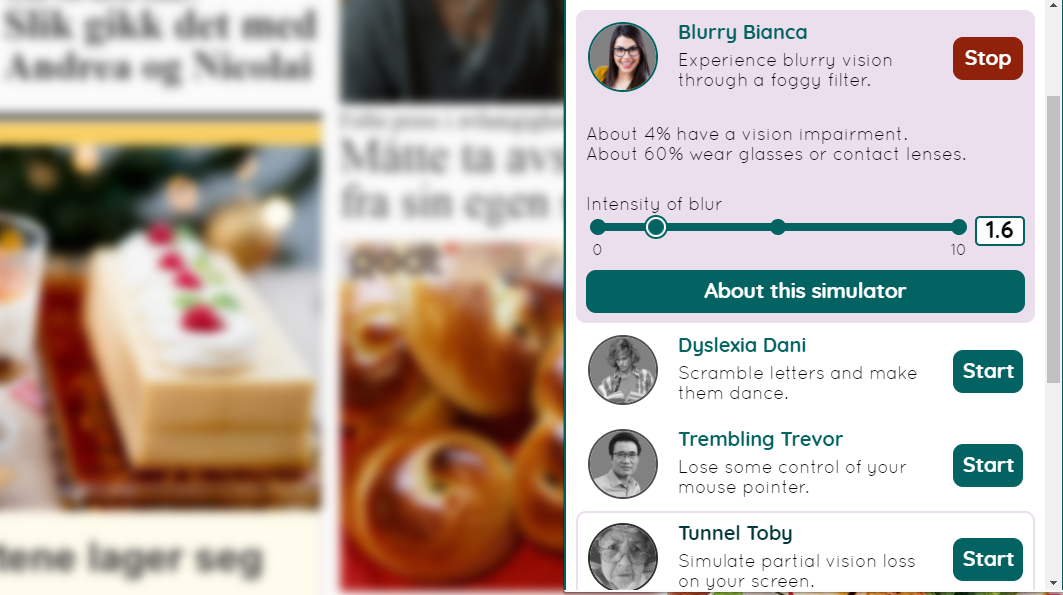
\includegraphics[width=\linewidth]{img/funkify_stats.png}
  \caption{\textit{Statistics are provided to quantify how many people are affected by each impairment.}}\label{fig:funkify_statistics}
\endminipage\hfill
\end{figure}

In figure \ref{fig:funkify_statistics} the persona "Blurry Bianca" is selected. The user of the simulator is provided information that around 4\% of the population has a vision impairment and that 60\% uses glasses or contact lenses. 


\section{Related work}
\subsection{Simulation in user-centred design: Helping designers to empathise with atypical users}
\textcite{Cardoso2012} says that designers often applies self-observation teqhniques when they design. This can lead to difficult, frustrating, dysfunctional or even dangerous interactions for a wider variety of people. People experiencing capability-losses, including old and people with temporary or permanent impairments, are likely to be most affected. A user-centered approach to design advocates for direct contact with end-users throughout the design process. 

However, sometimes clients might not think user involvement is a priority, and no allocation is made for it in the budget. Assessing with the use of user simulations has been used in times where user involvement can be hard to accomplish: 
\begin{displayquote}
    In the field of Inclusive/Universal Design, this has consisted of a person (usually able-bodied) wearing physical restrainers to feel the effects of different types of capability-losses, experienced for instance by people with impairments.
\end{displayquote}

Different impairments can be simulated:
